%!TEX root = ../../PhD_thesis__Edouard_Leurent

\graphicspath{{2-Chapters/2-Chapter/}}

\chapter{Literature Review}
\label{chapter:2}

\begin{flushright}
	\begin{tabular}{@{}l@{}}
		\emph{Souhaite que la route soit longue. [\dots]}\\
		\emph{Visite aussi beaucoup de villes égyptiennes,}\\
		\emph{et n’aie de cesse de t’instruire auprès de ceux qui savent.}\\
	\end{tabular}
	
	Konstantinos Kavafis, \href{https://eleurent.github.io/sisyphe/texts/ithaki.html}{\emph{Ithaque}}.
\end{flushright}

\section{Sequential decision-making}

TODO: take a series of driving decisions. The system is in a state $s\in\cS$, can take actions $a\in\cA$, leading to another state $s'\in S$. Actions are picked according to a policy $\pi(a|s)$, potentially stochastic. How to design this policy ?

\subsection{Motion Planning}

The development of motion planning techniques for intelligent vehicles date back to the late 80s, supported by international research projects such as Eureka (1987) of the Prometheus program, followed by the DARPA Grand and Urban Challenges (2004, 2007), and more recently the VIAC (2010), GCDC (2011) and Delphi (2015) challenges. In two surveys \citep{Gonzalez2016,Paden2016} studying the literature of this period, three main approaches have been identified.

\paragraph{Search-based algorithms}

This method involves forming a regular discrete partition of the reachable vehicle configurations $\cS$, called a \emph{lattice}. This framing reduces motion planning to the problem of finding a shortest path in a known graph. Then, traditional graph-search algorithms such as Dijkstra's algorithm \citep{Dijkstra1959}, $A^\star$ \citep{Hart1968} or $D^\star$ \citep{Stentz1994} can been used to compute the optimal trajectory. This technique has been applied by at least five different teams for driving on structured roads and unstructured parking during the DARPA Urban Challenge (Dijkstra for team Ben Franklin \citep{Bohren2008} and VictorTango \citep{Bacha2008}, and $A^\star$ for Stanford University \citep{Montemerlo2008} and KIT \citep{Kammel2008}, and $D^\star$ by the winning team from CMU \citep{Urmson2008}).

\begin{figure}[tp]
	\centering
	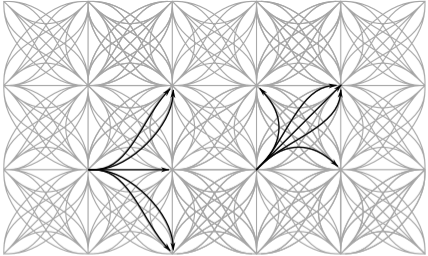
\includegraphics[width=0.5\linewidth]{img/lattice2}
	\caption{TODO: lattice}
\end{figure}

\paragraph{Sampling-based algorithms}

The limitation of search-based algorithms lies in the difficulty of formulating a regular lattice structure which feasible transitions between configurations, and in the real-time constraint that may not be met by graph-search algorithms. To address them, sampling-based motion planners iteratively grow a set of reachable configurations by randomly sampling valid transitions. The most popular ones are Probabilistic Roadmap (PRM), Rapidly-exploring Random Trees (RRT) and Monte-Carlo Tree Search algorithms.

\paragraph{Optimisation-based algorithms}

The third approach consists in optimizing a real-valued function parametrizing the trajectory. The most straightforward approach is curve fitting, which has been applied to various classes of functions in the context of Autonomous Driving, such as lines and circles, clothoids, polynomials, Bézier curves and splines.

Motion planning techniques thus rely on deterministic models of the kinematics or dynamics of the vehicle. These models are often required to take a simple form such that the search or optimisation procedure can be solved efficiently. Therefore, other objects are considered static and complex behaviours such as interactions between vehicles are left-out. Consequently, these techniques have mainly been successfully applied to the control of a single vehicle to track a sequence of known waypoints with static obstacles.

\subsection{Imitation Learning}

It may be the case that the vehicle position is not directly observed and only raw high-dimensional measurements such as camera images are available. As an effect, motion planning approaches that rely on models of the state dynamics are not applicable in these conditions. An orthogonal strategy is to learn a reactive mapping $\pi(a|s)$ under supervision of an expert $\pi_E$ that produces demonstration trajectories.

TODO: ref needed: dean pomerleau: ALVIN
\begin{figure}[tp]
	\centering
	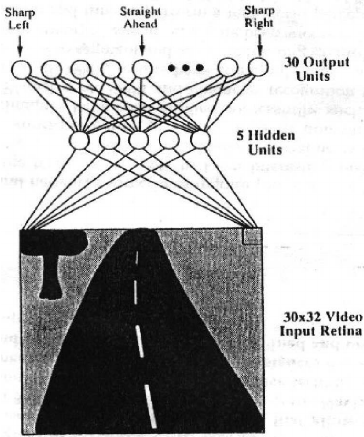
\includegraphics[width=0.4\linewidth]{img/alvinn}
	\caption{TODO: ALVIN}
\end{figure}

TODO: Compounding errors: \emph{"Supervised learning will not produce a policy with good long-horizon
performance, since a small mistake on the part of the policy will place the system
into states that are outside the distribution in the training data"} [Sergey Levine et al. “End-to-End Training of Deep Visuomotor Policies”. In: (2015).]

\begin{figure}[tp]
	\centering
	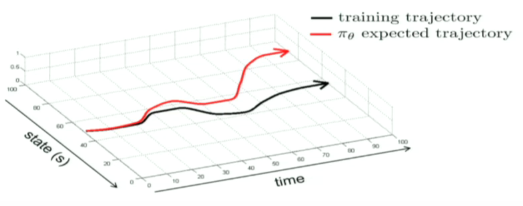
\includegraphics[width=0.7\linewidth]{img/cp4}
	\caption{TODO: Compounding errors}
\end{figure}

\subsection{Reinforcement Learning}
\section{States and partial observability}
\section{Actions and temporal abstraction}
\section{Rewards and inverse reinforcement learning}
\section{Dynamics and transfer}
\section{Optimisation criterion and safety}
